\chapter{Ecuaciones diofánticas}

\index{Ecuación!diofántica}
Una \textbf{ecuación diofántica} es una ecuación algebraica cuyos coeficientes
son números enteros y donde solamente interesan las soluciones enteras o quizá
las soluciones racionales. El nombre estas ecuaciones se debe al notable
matemático Diofanto. 

\begin{example}
	Comencemos con uno de los casos más sencillos de ecuaciones diofánticas
	lineales.  Sabemos que la ecuación 
	\[
		ax+by=c
	\]
	tiene solución en los enteros si y sólo si $c$ es un múltiplo del máximo
	común divisor entre $a$ y $b$.
\end{example}

Escribir el máximo común divisor $d$ entre $a$ y $b$ como $d=ra+sb$ para
enteros $r$ y $s$ se denomina comunmente la \emph{identidad de Bézout}. Este
resultado se conoce desde mucho tiempo antes, por lo menos desde 1624, ya que
aparece en un trabajo de Bachet de Méziriac.  Bézout demostró esa identidad
para polinomios en 1779.

Como sabemos, el cálculo del máximo común divisor entre dos enteros puede
hacerse mediante el \emph{algorithmo de división} (o el algoritmo de Euclides).
Este algoritmo es quizá el más antiguo que se conoce, y aparece formulado para
enteros en las proposiciones 1 y 2 del libro VII y para longitud de segmentos
en la proposiciones 2 y 3 del libro X de los Elementos. Hay mucha evidencia que
sugiere que el algoritmo de división no fue descubierto por Euclides sino que
era ya conocido por los pitagóricos y por Eudoxo. El algoritmo fue
redescubierto independiente en India y China y eso se hizo precisamente para
resolver ecuaciones diofánticas. 

Recordemos cómo funciona el algoritmo de división. Si queremos calcular el
máximo común divisor entre $840$ y $611$ hacemos el siguiente cálculo:
\begin{align*}
	& 840 = 1\times 611+229,\\
	& 611 = 2\times 229+153,\\
	& 229 = 1\times 153+76,\\
	& 153 = 2\times 76+1.
\end{align*}
Esto nos permite escribir las siguientes fracciones:
\begin{align*}
	&\frac{840}{611} = 1+\frac{229}{611}=1+\frac{1}{\frac{611}{229}},
	&&\frac{611}{229} = 2+\frac{153}{229}=2+\frac{1}{\frac{229}{153}},\\
	&\frac{229}{153} = 1+\frac{76}{153}=1+\frac{1}{\frac{153}{76}},
	&&\frac{153}{76} = 2+\frac{1}{76}.
\end{align*}
La fracción continua que representa al racional $840/611$ es entonces:
\[
	\dfrac{840}{611}=1+\dfrac{1}{2+\dfrac{1}{1+\dfrac{1}{2+\dfrac{1}{76}}}}.
\]

%Digamos que nos interesa resolver la ecuación
%\[
%	196+42y=28.
%\]
%Vamos a calcular el máximo común divisor entre $196$ y $42$. Primero calculamos 
%\begin{align*}
%	196 &= 42\times 4+28,\\
%	42 &= 28\times 1+14,\\
%	28 &= 14\times 2+0,
%\end{align*}
%y vemos que el máximo común divisor es $\gcd(196,42)=14$. Sabemos entonces
%que la solución\dots
%
%El número racional $196/42$ puede representarse por la fracción continua
%\[
%	\frac{196}{42}=4+\cfrac{1}{1+\cfrac{1}{1+\cfrac{1}{2}}}
%\]
%El matemático
%Indio Aryabhata las utilizó alrededor del año 500 para resolver ecuaciones
%diofánticas\dots

\begin{exercise}
	Resuelva $840x+611y=76$. 
\end{exercise}

\begin{exercise}
	Demuestre que la ecuación $8x+18y=1$ no tiene soluciones enteras.
\end{exercise}

\begin{example}
	La ecuación $x^2-2y^2=0$ no tiene soluciones en los enteros pues vimos que
	$\sqrt{2}$ no es un número racional. 
\end{example}

\begin{example}
	Sea $p$ un número primo.  De acuerdo con Hurwitz, Euler fue el primero en
	observar que la ecuación
	\[
		x^3+py^3+p^2z^3=0
	\]
	no tiene soluciones enteras no triviales. Supongamos que existe una
	solución $(x,y,z)$. Sin pérdida de generalidad podemos suponer que no todos
	estos números son divisibles por $p$. De la ecuación vemos que $p\mid x^3$,
	lo que implica que $p\mid x$. Si escribimos $x=pa$ y reemplazamos, la
	ecuación se transforma en 
	\[
		p^3a^3+py^3+p^2z^3=(pa)^3+py^3+p^2z^3=0.
	\]
	Al cancelar un $p$, nos queda $p^2a^3+y^3+pz^3=0$. Luego $p\mid y^3$ y en consecuencia $p\mid y$. Si escribimos
	$y=pb$ y reemplazamos, 
	\[
		p^2a^3+p^3b^3+pz^3=0.
	\]
	Al cancelar una $p$, obtenemos $pa^3+p^2b+z^3$. De aquí vemos que $p\mid
	z^3$ y luego $p\mid z$, una contradicción.
\end{example}

\begin{example}
En 1769 Euler conjeturó que la ecuación 
$x^4+y^4+z^4=w^4$,
o más generalmente 
\[
	x_1^k+x_2^k+\cdots+x_{k-1}^k=x_k^k,\quad
	k\geq4,
\]
no tiene soluciones enteras. 

Mediante un cálculo computacional más o menos directo, en 1966, Larden y Parkin
encontraron un contraejemplo para la conjetura de Euler en el caso $k=5$: 
\[
	27^5+84^5+110^5+133^5=144^5.
\]
Sin embargo, no pudieron encontrar contraejemplos para el caso $k=4$.  Más de
doscientos años después de aquella conjetura de Euler, en 1988, el matemático
estadounidense Noam Elkies encontró una infinidad de soluciones para la
ecuación de Euler en el caso $k=4$. Una de esas soluciones es 
\[
	2682440^4+15365639^4+18796760^4=20615673^4.
\]
No se sabe si la conjetura de Euler es verdadera si $k\geq6$. 

%Apenas unas semanas después del descubrimiento de Elkies, independientemente Zagier encontró 
%una solución de la ecuación de Euler.
\end{example}

\begin{example}
En 1946 Erd\"os y Straus conjeturaron que para cada entero $n\geq2$ existen
$x,y,z\in\N$ tales que 
\[
	\frac4n=\frac1x+\frac1y+\frac1z.
\]

\begin{exercise}
	Demuestre que solo es necesario demostrar la conjetura para los números primos
\end{exercise}
%La fórmula
%\[
%	\frac{4}{mp}=\frac{1}{ma}+\frac{1}{mb}+\frac{1}{mc}.
%\]
%implica que solamente necesitamos demostrar la conjetura para los $n$ que son
%números primos. 

\begin{exercise}
	Demuestre que la conjetura es verdadera para los primos $p$ tales que
	$p\equiv3\bmod 4$. 
\end{exercise}

Para $n=5$ la conjetura es verdadera pues 
\[
	\frac45=\frac12+\frac14+\frac1{20}.
\]
Más generalmente, si $n=3m+2$, siempre se tiene al menos una solución pues 
\[
	\frac4n=\frac1n+\frac{1}{(n+1)/3}+\frac{1}{n(n+1)/3}.
\]

Gracias al uso de computadoras se sabe que la conjetura es verdadera para todo
$n\leq10^{17}$.  La cantidad de soluciones para cada $n$ puede verse en la
sucesión \href{https://oeis.org/A073101}{A073101}. Al observar esta sucesión vemos que incluso si $n$ es
grande, la cantidad de soluciones es un número relativamente pequeño.  Al día
de hoy la conjetura está aún abierta. En 2013, Elsholtz y Tao obtuvieron un
avance importante en la conjetura de Erd\"os--Straus al lograr dar cotas para
la cantidad promedio de soluciones del problema. 
\end{example}


\index{Fracción!egipcia}
\index{Fracción!unitaria}
\index{Papiro!Ahmes}
\index{Papiro!Rhind}
\index{Papiro!de Moscú}
El ejemplo anterior involucra aquellas fracciones conocidas como
\textbf{fracciones egipcias}. Una fracción egipcia es una suma finita de
fracciones unitarias.  Todo racional positivo puede representarse por una
fracción egipcia; por esta razón los egipcios las utilizaban en las
aplicaciones prácticas.  A partir del estudio de algunos papiros, los
historiadores descubrieron algunos de los métodos con los que los egipcios
podían realizar cálculos con estas fracciones. 
Según Heródoto los egipcios son los padres de la geometría, aunque tenían una
matemática muy inferior a la matemática de los babilónicos.  
%Sabían calcular
%exactactamente áreas de triángulos, rectángulos y trapecios, y volúmenes de
%prismas y pirámides.  Tenían además una buena aproximación para el número
%$\pi$. Además del buen manejo que tenían de las fracciones, en los papiros
%aparecen operaciones elementales con enteros, progresiones aritméticas y
%geométricas y algunos ejemplos de raíces cuadradas. 

Este es un buen momento para hacer una pequeña digresión sobre la matemática
egipcia. Mucho de lo que sabemos de la matemática egipcia, se lo debemos a
antiguos papiros. Dos de los más famosos y más antiguos son el Papiro de Ahmes,
también conocido como el papiro matemático Rhind, y el Papiro de Moscú, ambos
del siglo XIX a. C. Estos dos papiros están formados por una colección de
problemas y recetas --con ejemplos numéricos concretos-- que permiten
resolverlos; y se creen fueron escritos para usarse como manuales de texto. Los
papiros contienen gráficos de sólidos geométricos, aunque  estos dibujos se ven
desde arriba o desde algún costado, ya que los egipcios no conocían la
perspectiva.  Entre los problemas incluidos en los papiros hay cálculo de áreas
de rectángulos, trapecios y triángulos. Aparece además la fórmula 
\[
	\frac{(a+c)}{2}\frac{(b+d)}{2}.
\]
que aproxima el área de un cuadrilátero de lados $a$, $b$, $c$ y $d$.  Es
interesante observar que esta fórmula también puede usarse para calcular área
de triángulos si alguno de los lados es igual a cero (como los egipcios no
conocían el número cero, simplemente sabían que para usar esta fórmula en
triángulos había que omitir uno de los lados). Según puede verse en los
papiros, para calcular el área de un círculo de diámetro $d$ usaban la
fórmula aproximada 
\begin{equation}
	\label{eq:egipcio_circle}
	\left(\frac89d\right)^2.
\end{equation}

No sabemos con exactitud cómo es que los egipcios consiguieron tal buena
aproximación, se cree que fue mediante la técnica de suscribir algún polígono
dentro del círculo.  Los papiros incluyen además cálculos exactos o aproximados
de algunos volúmenes cúbicos o cilíndricos.  Las pirámides egipcias sugieren
que los egipcios sabían calcular los volúmenes de esos sólidos geométricos,
aunque no disponemos de evidencia concreta. En 1910 el matemático alemán Dehn
observó que el cálculo del volumen de una pirámide requiere algún proceso de
paso al límite, técnica que los egipcios no disponían.  En el Papiro de Moscú
se explica que el volumen de una pirámide truncada de base cuadrada puede
calcularse con la fórmula
\[
	\frac{h}{3}(a^2+ab+b^2),
\]
donde $a$ es el lado de la base, $b$ es el lado del techo y $h$ es la altura de
la pirámide. 

\begin{example}
	Euler en 1770 demostró que $(5,3)$ es la única solución entera de la
	ecuación $y^3=x^2+2$. Esta ecuación ya había sido considerada por Diofanto
	en uno de sus libros, junto con la solución $(5,3)$. Fermat afirmó que
	$(5,3)$ era la única solución entera de la ecuación, aunque aquella
	demostración nunca fue publicada. 

	Para atacar este problema Euler consideró el conjunto
	\[
		\Z[\sqrt{-2}]=\{a+b\sqrt{-2}:a,b\in\Z\}.
	\]
	Al factorizar $y^3=(x+\sqrt{-2})(x-\sqrt{-2})$ obvervó que si los elementos
	de $\Z[\sqrt{-2}]$ fueran como los números enteros, entonces los números
	$x+\sqrt{-2}$ y $x-\sqrt{-3}$ también serían cubos. En particular, como
	\[
		x+\sqrt{-2}=(a+b\sqrt{-2})^3,
	\]
	para ciertos $a,b\in\Z$, tendríamos entonces
	\[
		x+\sqrt{-2}=a^3-6ab^2+(2a^2b-2b^3)\sqrt{-2}.
	\]
	Esta igualdad implica entonces que $x=a^3-6ab^2$ y que $1=b(3a^2-2b^2)$. 
	De aquí se obtiene inmediatamente que $b\in\{-1,1\}$ y que $3a^2-2b^2\in\{-1,1\}$. 
	En consecuencia, $(5,3)$ es la única solución de la
	ecuación $y^3=x^2+2$. La demostración de Euler no es del todo correcta, ya
	que nunca demostró por qué es posible considerar a los elementos del
	conjunto $\Z[\sqrt{-2}]$ como números que son casi como los enteros.
\end{example}

El argumento de Euler del ejercicio anterior es esencialmente correcto, pero
hay cosas que requieren una justificación rigurosa.  Más aún, si esta ingeniosa
técnica de Euler no es utilizada con cuidado, nos llevará inevitablemente a
conclusiones incorrectas. Si consideramos, por ejemplo, que los elementos de
$\Z[\sqrt{-5}]$ son también números como los números enteros, podríamos
``demostrar'' entonces que la ecuación $y^2=x^2-5$ no tiene soluciones enteras,
algo claramente falso pues $(x,y)=(3,2)$ es una solución.  

Los ``enteros'' de la forma $a+b\sqrt{n}$, donde $n$ es algún entero libre de
cuadrados, que mencionamos anteriormente son casos particulares de algo que hoy
conocemos bajo el nombre de \emph{enteros algebraicos}. La teoría de estos
números fue ampliamente desarrollada entre 1840 y 1850 gracias al trabajo de
Dirichlet, Kummer, Eisenstein, Hermite, Kronecker, etcétera. Estos enteros juegan un
papel fundamental en la resolución de ciertas ecuaciones diofánticas, y en
particular en la ecuación diofántica más famosa: aquella que da lugar el
teorema de Fermat.

\section*{El teorema de Fermat}

Ya sabemos que construir ternas pitagóricas es encontrar
soluciones enteras de la ecuación 
\[
	x^2+y^2=z^2.
\]
Esta ecuación puede generalizarse en varias direcciones, una de estas
generalizaciones nos lleva al famoso \emph{teorema de Fermat}.  

Si bien Fermat
hizo muchas contribuciones a la matemática, esta sección se refiere a un
resultado ``conjeturado'' por Fermat en 1637 y demostrado por Wiles en 1995. El
teorema afirma que no existen soluciones enteras no triviales de la ecuación
\[
	x^n+y^n=z^n
\]
para $n\geq3$. 

El resultado fue escrito por Fermat en los márgenes de una copia de un libro de
Diofanto, acompañado por una frase que decía que, en esos márgenes, no había
espacio suficiente que pudieran contener la maravillosa demostración que él
había encontrado.  Durante mucho tiempo muchos matemáticos de gran nombre
intentaron en vano demostrar que no existen soluciones no triviales. La lista
de nombres es larga: Euler, Legendre, Gauss, Abel, Cauchy, Dirichlet, Lamé,
Kummer, Frobenius, Furtwangler, Dickson, etcétera.

Fermat lo demostró en el caso $n=4$ y para esto utilizó un precursor del
principio de inducción conocido como ``el método del descenso''. En realidad,
Fermat demostró algo un poquito más general. Para demostrar este resultado de
Fermat necesitamos primero demostrar el siguiente lema:

\begin{lemma}
	\label{lem:cuadrados}
	Si $u$ y $v$ son enteros coprimos tales que $uv$ es un cuadrado, entonces
	$u$ y $v$ son también cuadrados.
\end{lemma}

\begin{proof}
	Escribimos $u=p^{\alpha}m$ donde $p$ es un primo que divide a $u$ y $m$ no
	es divisible por $p$. Como $uv=p^{\alpha}t$ para algún entero $t$ no
	divisible por $p$ y $uv$ es un cuadrado, el exponente $\alpha$ es un número
	par. Como este razonamiento puede hacerse para cualquier primo que divide a
	$u$, se concluye que $u$ es un cuadrado. Análogamente se demuestra que $v$
	es también un cuadrado. 
\end{proof}

Ahora sí estamos en condiciones de demostrar el siguiente resultado:

\begin{theorem}
	La ecuación $x^4+y^4=z^2$ no tiene soluciones enteras positivas.
\end{theorem}

\begin{proof}
	Supongamos que el resultado no es cierto. Sean entonces	$x,y,z$ enteros
	positivos tales que $x^4+y^4=z^2$, donde entre todas estas posibles ternas
	nos quedamos con aquella donde $z$ es mínimo entero positivo posible. Como
	entonces $x^2,y^2,z$ forman una terna pitagórica primitiva, podemos suponer
	sin perder generalidad que $x^2$ es impar e $y^2$ es par, recordemos el
	ejercicio~\ref{xca:paridad}. Por el teorema~\ref{thm:ternas_pitagoricas}
	sabemos que entonces
	\[
		x^2=m^2-n^2,\quad
		y^2=2mn,\quad
		z=m^2+n^2
	\]
	para ciertos enteros positivos coprimos $m,n$ tales que $m\not\equiv n\bmod
	2$. La primera fórmula nos dice además que $x,n,m$ es también una terna
	pitagórica primitiva, y en consecuencia, como $x$ es impar, podemos
	escribir
	\[
		x=r^2-s^2,\quad
		n=2rs,\quad
		m=r^2+s^2
	\]
	para ciertos enteros positivos coprimos $r,s$ tales que $r\not\equiv s\bmod
	2$. La tercera ecuación es $m=r^2+s^2$ y nos dice que entonces los enteros
	$r$, $s$ y $m$ serán coprimos dos a dos (pues recordemos que $r$ y $s$ son
	coprimos). Como
	\[
		y^2=2mn=4mrs
	\]
	y los enteros $r$, $s$ y $m$ son coprimos dos a dos, el lema anterior nos
	permite demostrar que existen $a,b,c\in\N$ tales que $r=a^2$, $s=b^2$,
	$m=c^2$. Como $m=r^2+s^2$, 
	\[
		c^2=a^4+b^4,
	\]
	donde $c\leq c^4=m^2< m^2+n^2=z$, una contradicción a la minimalidad de
	$z$.
\end{proof}

\begin{exercise}
	Demuestre que la ecuación $x^4+y^4=z^4$ no tiene soluciones enteras
	positivas.
\end{exercise}

%\begin{proof}
%	Una solución de la ecuación del enunciado sería también una solución de la
%	ecuación que tenemos en el teorema anterior.
%\end{proof}

\begin{exercise}
	Demuestre que debe demostrarse la afirmación hecha por Fermat solamente en
	el caso en que el exponente sea un primo impar.
\end{exercise}

En 1770 Euler dio una demostración incorrecta para el caso $n=3$. La
demostración dada por Euler asume que los números de la forma
\[
	a+b\sqrt{-3}
\]
con $a$ y $b$ enteros, se portan tal como se portan los enteros, cosa que en
realidad no es cierta, ya que los elementos de $\Z[\sqrt{-3}]$ no admiten
factorización única como producto de primos (en $\Z[\sqrt{-3}])$. La
demostración del caso $n=3$ puede repararse y eso se hace utilizando ciertas
técnicas que aparecen en los trabajos de Euler. Por esa razón, no está del todo
mal afirmar que Euler fue el que logró demostrar el caso $n=3$. 

Después de esos primeros resultados no hubo grandes avances sino hasta que
apareció Sophie Germain. Ella observó que los primos $p$ tales que $2p+1$ es
también un número primo eran relevantes para desarrollar una estrategia que
permitiera atacar el problema de Fermat.  Hizo varias contribuciones en esta
dirección que luego fueron extendidas por Legendre. 

\index{Primos!de Germain}
Los números primos $p$ tales que $2p+1$ es también un número primo hoy son
conocidos como los \textbf{primos de Germain}. 
Los primeros primos de Germain
son
\[
	2, 3, 5, 11, 23, 29, 41, 53, 83, 89, 113, 131, 173, 179, 191, 233, 239,
	251\dots
\]
y podemos verlos en la sucesión 
\href{https://oeis.org/A005384}{A005384}.
Hoy en día estos números primos
tienen aplicaciones en criptografía. Se conjetura que existen infinitos primos
de Germain; el mayor primo de Germain conocido es 
\[
	2618163402417\times 2^{1290000} - 1,
\]
un número de 388342 dígitos. Este primo fue encontrado en febrero de 2016
gracias a un proyecto de cálculo distribuido del que hablaremos en el capítulo
sobre números primos. 

En 1832 Dirichet, en un intento por atacar el caso $n=7$, publicó una
demostración del caso $n=14$. El caso $n=7$ fue finalmente demostrado por Lamé
en 1839 con métodos completamente distintos a los de Dirichlet. La dificultad
de la demostración encontrada por Lamé contribuyó a alimentar la creencia de
que nuevas ideas iban a ser necesarias para lograr atacar el problema de Fermat
para exponentes arbitrarios. 

En 1847 Lamé anunció haber demostrado el problema de Fermat con total
generalidad. Su demostración se basaba en poder factorizar $x^n+y^n$ en
factores lineales sobre los números complejos, 
\[
	x^n+y^n=(x+y)(x+\zeta y)(x+\zeta^2y)\cdots (x+\zeta^{n-1}y),
\]
donde $\zeta$ es una raíz $n$-ésima primitiva de la unidad. 
Según Lamé, la idea basada en aquella 
factorización viene de Liouville. Sin embargo, fue Liouville uno de los
primeros en observar que para que el argumento de Lamé funcionara correctamente
era necesario disponer de resultados de factorización única como producto de
primos, cosa que para él en general no siempre existiría. Durante las semanas
siguientes muchos matemáticos intentaron demostrar aquella unicidad. Wantzel,
por ejemplo, afirmó haber demostrado tal unicidad al mencionar que el resultado
era cierto para $n\in\{2,3,4\}$ y que uno fácilmente podría utilizar el mismo
argumento para tratar cualquier $n>4$. Obviamente Wantzel estaba equivocado,
recordemos que el error cometido por Euler en el caso $n=3$ era exactamente
suponer una factorización única donde no existe. Poco tiempo después Kummer
envió una carta en donde demostraba que la factorización
única no siempre es posible: mostró que
\[
	(4+\sqrt{-5})\times (4-\sqrt{-5})=3\times 7=21
\]
permite factorizar al número $21$ como producto de ``primos'' de
$\Z[\sqrt{-5}]$ en, al menos, dos formas distintas. Paralelamente Kummer
introdujo entonces una nueva teoría para reemplazar los problemas encontrados
por culpa de aquella falta de unicidad en la factorización como producto de
primos. Esa nueva teoría dio origen a una cierta clase de números primos, los
\textbf{primos regulares}. 

\index{Primos!regulares}
Para esos primos Kummer Kummer resolvió el problema de Fermat.  Los primeros
primos regulares impares son
\[
    3, 5, 7, 11, 13, 17, 19, 23, 29, 31, 41, 43, 47, 53, 61, 71, 73\dots
\]
y aparecen en la sucesión \href{https://oeis.org/A007703}{A007703}. No se sabe si hay infinitos primos
regulares. 

En 1915 Jensen demostró que hay infinitos primos irregulares (es
decir, no regulares).  

En 1965 Siegel conjeturó que hay infinitos primos
regulares y que representan aproximadamente el 60\% del total de los primos.

A mediados del siglo XX la matemática comenzó a transitar ciertos caminos que
unos cincuenta años más tarde permitirían resolver con total generalidad el
problema de Fermat. 

En 1983 Faltings demostró que para cada $n$ existen a lo
sumo finitas soluciones de la ecuación $x^n+y^n=z^n$, obtuvo esto como
consecuencia de haber demostrado una conjetura hecha por Mordell en 1922 sobre
la existencia de puntos racionales en curvas. 

En 1986 Frey observó que la
existencia de una terna $(a,b,c)$ de enteros positivos tales que $a^n+b^n=c^n$
podría implicar un fenómeno muy particular, conocido como \emph{no
modularidad}, para la curva
\[
	y^2=x(x-\alpha)(x-\beta),
\]
donde $\alpha$ y $\beta$ son ciertos enteros que dependen de $a$ y $b$. 
Ese fenómeno de no modularidad construido a partir de posibles
contraejemplos fue luego demostrado por Ribet en 1990. La no modularidad es, en
realidad, imposible. Este resultado, demostrado por Wiles en 1995, da 
entonces una solución completa del problema de Fermat.
La demostración es extremadamente difícil y utiliza
técnicas sofisticadas pertenecientes a distintas áreas de la matemática.  

\section*{La ecuación de Pell}

\index{Ecuación!de Pell}
En este capítulo veremos un poco de historia sobre una ecuación diofántica muy
famosa, la ecuación de Pell:
\begin{equation}
	\label{eq:Pell}
	x^2-Ny^2=1.
\end{equation}
Nos interesan las soluciones enteras, es decir soluciones $(x,y)\in\Z\times\Z$.
Hay soluciones triviales, son $(x,y)=(1,0)$ y $(x,y)=(-1,0)$. Una solución
$(x,y)$ de la ecuación~\eqref{eq:Pell} se dirá positiva si $x>0$ e $y>0$. Nos
concentraremos entonces en la existencia de soluciones positivas de la ecuación
de Pell.

\begin{exercise}
	Demuestre que si $N$ es un cuadrado, la ecuación~\eqref{eq:Pell} solo
	tiene soluciones triviales.
\end{exercise}

Podemos encontrarnos a la ecuación de Pell o ecuaciones similares en India y
Grecia, donde se logró conseguir aproximaciones racionales para ciertas raíces
cuadradas gracias a soluciones de la ecuación de Pell. 
Cerca del año 400 a.C., el matemático
indio Baudh\=ayana consigue aproximar al número $\sqrt{2}$ con las fracciones
$17/12$ y $577/408$. Observemos que 
\[
%	\frac{17}{12}+\frac{-1}{2\times 12\times 17}=\frac{577}{408},\quad
	17^2-2\times 12^2=1,\quad
	577^2-2\times 408^2=1.
\]
Siglos después Arquímedes observó que el irracional $\sqrt{3}$ puede
aproximarse con los racionales $265/153$ y $1351/780$. Observar que
\[
	265^2-3\times 153^2=-2,\quad
	1351^2-3\times 780^2=1. 
\]
Veremos que esta
conexión entre la aproximación de irracionales y la ecuación de Pell resultará
de fundamental importancia a la hora de entender cómo pueden construirse
soluciones de esta famosa ecuación.  
	
%El método para resolver~\eqref{eq:Pell} de Brouncker es similar 
%al que ya conocían los matemáticos indios del siglo X; Euler reformuló el
%método en términos de fracciones continuas.  
Se cree que Fermat tenía una demostración de que la ecuación de Pell siempre
tiene solución en los enteros positivos; de hecho, en una carta desafió a otros
matemáticos a que intentaran al menos resolver las ecuaciones de Pell con
$N=61$ y $N=109$.  Euler se interesó en la ecuación de Pell al preguntarse qué
relaciones podían existir entre distintos números poligonales.  Entre 1766 y
1769 Lagrange trabajó con esta ecuación y fue el primero en demostrar que la
ecuación de Pell tiene soluciones no triviales siempre que $N$ no sea un
cuadrado perfecto. 

\begin{example}
	Los números que son simultáneamente cuadrados y triangulares se
	corresponden con soluciones de la ecuación $x^2-2y^2=1$. En efecto, si $n$
	es triangular y es además un cuadrado, podemos escribir 
	\[
		\frac{k(k+1)}{2}=l^2
	\]
	para $k,l\in\N$, y esta última fórmula es equivalente a
	$(2k+1)^2-2(2l)^2=1$.
\end{example}

%\begin{exercise}
%	Demuestre que de la misma forma puede relacionarse la ecuación $x^2-6y^2=1$
%	con números que son simultáneamente triangulares y pentagonales.
%\end{exercise}

Fermat sabía que la ecuación $x^2-61y^2=1$ es particularmente difícil de
resolver. La solución $(x,y)$ con el menor positivo entero positivo $y$ es
\[
(x,y)=(1766319049, 226153980).
\]

\begin{exercise}
	Demuestre que si $(x,y)$ es una solución de la ecuación de Pell, entonces 
	$(x^2+Ny^2,2xy)$ es también una solución de la ecuación de Pell. 
\end{exercise}

\begin{exercise}
	Demuestre que si la ecuación de Pell tiene al menos una solución no
	trivial, entonces tendrá infinitas soluciones. 
\end{exercise}

Veamos cómo fue que los matemáticos indios pudieron resolver esta ecuación.  En
el año 628 Brahmagupta resolvió la ecuación de Pell para muchos $N$  pero no
para todos. En el siglo IX Jayadeva mejoró el método de Brahmagupta y concibió
el ``método cíclico''. Este método fue perfeccionado en el siglo XII por
Bhaskara II. 

\index{Método!cíclico}
\index{Identidad!de Brahmagupta}
El ``método cíclico'' funciona de la siguiente manera. 
Diremos que $(a,b,N)$ es una \textbf{terna de Pell}
si $a^2-Nb^2=1$. La identidad de Brahmagupta, 
\begin{equation}
	\label{eq:brahmagupta}
	(x_1^2-Ny_1^2)(x_2^2-Ny_2^2)=(x_1x_2+Ny_1y_2)^2-N(x_1y_2+x_2y_1)^2,
\end{equation}
entonces, nos permite combinar las ternas $(x_1,y_1,k_1)$ y $(x_2,y_2,k_2)$ en
una nueva terna $(x_1x_2+Ny_1y_2,x_1y_2+x_2y_1,k_1k_2)$ para todo $N$. En
particular, si $(a,b,k)$ es una terna de Pell, podemos combinarla con cualquier
$(m,1,m^2-N)$ para obtener la ternas de Pell de la forma
$(am+Nb,a+bm,k(m^2-N))$.

\begin{exercise}
	Demuestre la identidad~\eqref{eq:brahmagupta} de Brahmagupta.
\end{exercise}

Sea $(a,b)$ una solución de $x^2-Ny^2=k$, donde $a$ y $b$ son coprimos y $k$ es
algún número entero cualquiera. Elegiremos este $k$ de forma que sea fácil
conseguir $a$ y $b$. Lo que dijimos antes implica que
\begin{equation}
	\label{eq:Pell_inductive}
	\left(\frac{am+Nb}{k}\right)^2-N\left(\frac{a+bm}{k}\right)^2=\frac{m^2-N}{k}
\end{equation}
para todo $m\in\N$. 
Si elegimos $m$ para que $\frac{a+bm}{k}$ sea un entero y que minimice la
expresión $m^2-N$, tenemos una nueva solución a otra ecuación de Pell. Podemos
entonces repetir este procedimiento tantas veces como sea necesario hasta
obtener una ecuación de Pell de la forma $a^2-Nb^2=1$. ¡Resolvimos entonces la ecuación original!

\begin{exercise}
	Encuentre soluciones para $x^2-14y^2=1$ con el método cíclico. 
\end{exercise}

%Veamos cómo este método nos permite resolver eficientemente la ecuación
%$x^2-61y^2=1$.  Comencemos con la ecuación $x^2-61y^2=3$. A simple vista puede
%verse que $(8,1)$ es una solución no trivial, y entonces tenemos la terna de
%Pell $(8,1,3)$. Si componemos esta terna con alguna terna de Pell de la forma
%$(m,1,m^2-61)$, obtenemos la terna de Pell $(8m+61,8+m,3(m^2-61))$. Al dividir,
%tenemos la terna de Pell
%\[
%	\left(\frac{8m+61}{3},\frac{8+m}{3},\frac{m^2-61}{3}\right).
%\]
%Tenemos que elegir $m$ para que $\frac{m^2-61}{3}\in\Z$ y que minimice
%$m^2-61$, y basta con tomar $m=7$. Así es que tenemos entonces la terna de Pell
%$(39,5,-4)$, que al combinar con $(m,1,m^2-61)$ nos permite construir la terna 
%\[
%	\left(\frac{}{},\frac{}{},\frac{}{}\right),
%\]
%que es la terna~\eqref{eq:Pell_inductive} con $a=39$, $b=5$, $k=-4$, $m=7$ y $N=61$. 
Otro método que permite resolver la ecuación de Pell es el método de Lagrange,
que fue reformulado por Euler en términos de fracciones continuas. 
%Si queremos resolver $x^2-61y^2=1$ con el método de las fracciones continuas, necesitamos 
%calcular la representación del número irracional $\sqrt{61}$ como fracción
%continua: 
%\[
%	\sqrt{61}=7+\cfrac{1}{1+\cfrac{1}{4+\cfrac{1}{3+\cdots}}}
%\]
%
%\begin{exercise}
%	Calcule la fracción continua que representa a $\sqrt{61}$. ¿Cuál es su
%	período?  Podemos ver esta representación en la sucesión \verb+A010145+.
%\end{exercise}
%
Veamos cómo funciona el método por fracciones continuas en el caso
\begin{equation}
	\label{eq:Pell14}
	x^2-14y^2=1.
\end{equation}
Primero calculamos la fracción continua que representa a $\sqrt{14}$, que será
periódica con período igual a cuatro:
\[
	\sqrt{14}=3+\cfrac{1}{1+\cfrac{1}{2+\cfrac{1}{1+\cfrac{1}{3+\sqrt{14}}}}}.
\]
El método explica cómo proceder en caso de que el período sea par o impar. En
nuestro caso, debemos trucar esta aproximación al final del primer período.
Obtenemos así una buena aproximación racional para $\sqrt{14}$, 
\[
	\sqrt{14}\sim 3+\cfrac{1}{1+\cfrac{1}{2+\cfrac{1}{1}}}=\cfrac{15}{4}.
\]
Esta fracción nos da además la solución $(x_1,y_1)=(15,4)$ de la
ecuación~\eqref{eq:Pell14}.  Podemos conseguir otras soluciones al calcular
\[
	x_n+y_n\sqrt{14}=(x_1+y_1\sqrt{14})^n.
\]

Es interesante observar que 
la fórmula anterior nos permite definir recursivamente soluciones de la
ecuación de Pell:
\begin{align*}
	x_{k+1} &= x_1x_k+Ny_1y_k,\\
	y_{k+1} &= x_1y_k+Ny_1x_k.
\end{align*}

\begin{exercise}
	Sea $n\in\N$.  Demuestre que si $(r,s)$ es una solución de la ecuación de
	Pell y el par $(u,v)$ está dado por la fórmula 
	\[
		u+v\sqrt{N}=(r+s\sqrt{N})^n,
	\]
	entonces $(u,v)$ es solución de la ecuación de Pell.
\end{exercise}

Vimos en el capítulo sobre números irracionales que Dirichlet demostró que si
$\alpha$ es un número irracional, existen infinitos números racionales $p/q$
tales que
\[
	\left|\alpha-\frac{p}{q}\right|<\frac{1}{q^2}.
\]
Este resultado le permitió a Dirichlet en 1842 obtener una demostración
alternativa de aquel resultado demostrado por Lagrange, que nos dice que la
ecuación de Pell siempre admite una solución no trivial. 

Para demostrar esto, primero comenzaremos con un lema que utiliza una versión
infinita del \emph{principio del palomar}: si infinitos elementos se
distribuyen en un número finito de cajas, entonces alguna caja contendrá
infinitos elementos.

\begin{lemma}
	Sea $N$ un entero que no es un cuadrado.  Existe entonces un entero $k$ con
	$|k|<2\sqrt{N}+1$ tal que la ecuación 
	\[
		x^2-Ny^2=k
	\]
	admite infinitas soluciones enteras. 
\end{lemma}

\begin{proof}
	Como $\alpha=\sqrt{N}$ es un número irracional, el teorema de Dirichlet nos
	permite encontrar una cantidad infinita de racionales $p/q$ tales que
	\[
		\left|\alpha-\frac{p}{q}\right|<\frac{1}{q^2}.
	\]
	Como entonces 
	\[
		\frac{p}{q}<\alpha+\frac{1}{q^{2}}<\alpha+1,
	\]
	tenemos 
	\begin{align*}
		|p^2-Nq^2|&=q^2\left|\sqrt{N}-\frac{p}{q}\right|\left|\sqrt{N}+\frac{p}{q}\right|
		<q^2\frac{1}{q^2}\left|\sqrt{N}+\frac{p}{q}\right|<2\sqrt{N}+1.
	\end{align*}
	En particular, esto nos dice que la expresión $|p^2-Nq^2|$ solamente tomará
	una cantidad finita de valores, y estos valores serán enteros $k$ tales que
	\[
		-2\sqrt{N}-1<k<2\sqrt{N}+1. 
	\]
	Estamos en condiciones entonces de utilizar la variante del principio del
	palomar que mencionamos anteriormente: tenemos infinitos racionales $p/q$ y
	finitos $k$ tales que $|p^2-Nq^2|=k$. En consecuencia, existirá algún $k$
	tal que infinitas fracciones $p/q$ satisfacen $|p^2-Nq^2|=k$.
\end{proof}

Consideremos el conjunto $\Z[\sqrt{N}]$ de números de la forma $u+v\sqrt{N}$
donde $u$ y $v$ son números enteros.  Para cada
$\alpha=u+v\sqrt{N}\in\Z[\sqrt{N}]$ definimos su norma como
$N(\alpha)=u^2-Nv^2$. 

\begin{exercise}
	\label{xca:Pell}
	Demuestre que si $\alpha\in\Z[\sqrt{N}]$ y $N(\alpha)=1$, entonces
	$\alpha^{-1}\in\Z[\sqrt{N}]$. Más generalmente, si $\alpha=u+v\sqrt{N}$,
	entonces
	\[
		\alpha^{-1}=\frac{u-v\sqrt{N}}{N(\alpha)}.
	\]
\end{exercise}

\begin{exercise}
	Demuestre si $\alpha,\beta\in\Z[\sqrt{N}]$, entonces
	$N(\alpha\beta)=N(\alpha)N(\beta)$.
\end{exercise}

Los ejercicios anteriores resultarán de gran utilidad a la hora de resolver la
ecuación de Pell. Nos permiten, además, entender conceptualmente la identidad
de Brahmagupta~\eqref{eq:brahmagupta}. 

\begin{theorem}[Lagrange]
	Sea $N$ un entero que no es un cuadrado. La ecuación $x^2-Ny^2=1$ admite al
	menos una solución positiva. 
\end{theorem}

\begin{proof}
	Gracias al lema anterior sabemos que existe $k$ tal que la ecuación
	$x^2-Ny^2=k$ tiene infinitas soluciones. Sean $(x_1,y_1)$ y $(x_2,y_2)$ dos
	soluciones distintas de esta ecuación. Podemos suponer sin perder generalidad que
	$x_1\equiv x_2\bmod{|k|}$ y que $y_1\equiv y_2\bmod{|k|}$ (pues existen
	$k^2$ posibilidades para elegir $x$ e $y$ módulo $|k|$ y existen infinitas
	soluciones). Para cada $i\in\{1,2\}$ sea 
	\[
		\alpha_i=x_i+\sqrt{N}y_i.
	\]
	Sea $\beta=\alpha_1\alpha_2^{-1}$. Calculamos 
	\[
		u^2-Nv^2=N(\beta)=N(\alpha_1\alpha_2^{-1})=N(\alpha_1)N(\alpha_2)^{-1}=1 
	\]
	y observamos que si podemos demostrar que $u,v\in\Z$, entonces $(u,v)$ será
	una solución de la ecuación de Pell. Veamos que efectivamente $u,v\in\Z$.
	Calculamos 
	\[
		\beta=(x_1+y_1\sqrt{N})\frac{x_2-y_2\sqrt{N}}{k}
		=\frac{x_1x_2-Ny_1y_2}{k}+\frac{x_1y_2-x_2y_1}{k}\sqrt{N},
	\]
	y vemos entonces que
	\[
	u=\frac{x_1x_2-Ny_1y_2}{k},
	\quad
	v=\frac{x_1y_2-x_2y_1}{k}\sqrt{N}.
	\]
	Como 
	sabemos que $x_1\equiv x_2\bmod{|k|}$ e $y_1\equiv y_2\bmod{|k|}$, tenemos que
	\[
		x_1x_2-Ny_1y_2\equiv x_1^2-Ny_1^2\equiv 0\bmod {|k|},\quad
		x_1y_2-x_2y_1\equiv 0\bmod{|k|}.
	\]
	Veamos que la solución que encontramos es no trivial: si $(u,v)=(1,0)$,
	entonces $1=\beta=\alpha_1\alpha_2^{-1}$ y luego $\alpha_1=\alpha_2$, una
	contradicción.
\end{proof}

Lo que vimos sobre la ecuación de Pell nos permite entonces demostrar el
siguiente resultado, obtenido por Lagrange. Ya vimos que la ecuación de Pell 
\[
	x^2-Ny^2=1
\]
siempre admite al menos una solución no trivial. Definimos
entonces a la \textbf{solución fundamental} de la ecuación de Pell como aquella
solución $(r,s)$ donde $s$ es el menor entero positivo posible, es
decir que vale $0<s<v$ para toda solución $(u,v)$ de enteros
positivos de la ecuación de Pell.

\begin{theorem}[Lagrange]
	Si $(r,s)$ es la solución fundamental de la ecuación de Pell, entonces toda
	solución de la ecuación de Pell
	puede escribirse como $(a,b)$, donde
	\[
		a+b\sqrt{N}=(r+s\sqrt{N})^k
	\]
	para algún entero positivo $k$. 
\end{theorem}

\begin{proof}
	Si suponemos que el resultado no es cierto, existirá un entero positivo $k$
	tal que
	\[
		(r+s\sqrt{N})^k<a+b\sqrt{N}<(r+s\sqrt{N})^{k+1}.
	\]
	Como $N(r+s\sqrt{N})=r^2-Ns^2=1$, el ejercicio~\ref{xca:Pell} nos 
	dice que 
	\[
		(r+s\sqrt{N})^{-k}=(r-s\sqrt{N})^k, 
	\]
	y esto nos permite reescribir la desigualdad anterior como
	\[
		1<(a+b\sqrt{N})(r+s\sqrt{N})^{-k}<r+s\sqrt{N}.
	\]
	Sea $\alpha=u+v\sqrt{N}=(a+b\sqrt{N})(r+s\sqrt{N})^{-k}$. Entonces
	$(u,v)$ es una solución de la ecuación de Pell
	pues 
	\begin{align*}
		u^2-Nv^2&=N(u+v\sqrt{N})\\
		&=N(a+b\sqrt{N})N(r+s\sqrt{N})^{-k}\\
		&=(a^2-b^2\sqrt{N})(r^2-s^2\sqrt{N})^{-k}=1.
	\end{align*}
	Por otro lado, como $\alpha^{-1}=u-v\sqrt{N}$, entonces $0<u-v\sqrt{N}<1$.
	Como además $1<u+v\sqrt{N}$, tenemos entonces que $u$ y $v$ son ambos
	positivos pues 
	\begin{align*}
		2u&=(u+v\sqrt{N})+(u-v\sqrt{N})>1+0>0,\\
		2v\sqrt{N}&=(u+v\sqrt{N})-(u-v\sqrt{N})>1+(-1)=0.
	\end{align*}
	Por la minimalidad de $(r,s)$, tenemos que $u\geq r$, pero entonces $u<r$ pues 
	\[
		u+s\sqrt{N}\leq u+v\sqrt{N}<r+s\sqrt{N}.
	\]
	Esto implica que $v<r$ pues 
	\[
		v^2=\frac{u^2-1}{N},\quad
		s^2=\frac{r^2-1}{N},
	\]
	una contradicción.
\end{proof}


\index{Problema!del ganado}
%La historia sobre la ecuación de Pell es fascinante y hay muchas cosas para aprender sobre 
%este tema~\cite{MR734177}. 
Terminaremos la sección con una historia muy interesante
que involucra a Arquímedes. 
Un bibliotecario de nombre 
Lessing encontró, en agosto 1773, en una biblioteca 
de Wolfenbüttel, Alemania, un manuscrito que contenía una carta dirigida a
Eratóstenes. El manuscrito, escrito en forma de poema, plantea el
problema de calcular el número de reses del mitológico rebaño de Sol, citado en
la Odisea, sabiendo que está sujeto a un conjunto de restricciones.  El
problema involucra resolver un caso particular de la ecuación de
Pell. El enunciado, según Wikipedia, es más o menos así:

\begin{quote}
	El dios sol tenía un rebaño formado por un cierto número de toros blancos,
	negros, moteados y amarillos, así como vacas de los mismos colores. De tal
	forma que: El número de toros blancos es la mitad y la tercera parte de los
	negros más los amarillos.  El número de toros negros es igual a la cuarta
	más la quinta parte de los moteados más los amarillos.  El número de toros
	moteados es igual a la sexta más la séptima parte de los blancos más los
	amarillos.  El número de vacas blancas es igual a un tercio más un cuarto
	de la suma de los toros negros y las vacas negras.  El número de vacas
	negras es igual a la cuarta parte más la quinta parte de la suma de los
	toros moteados más las vacas moteadas.  El número de vacas moteadas es
	igual a la quinta más la sexta parte de la suma de los toros amarillos más
	las vacas amarillas.  El número de vacas amarillas es igual a la sexta más
	la séptima parte de la suma de los toros blancos más las vacas blancas. La
	suma de los toros blancos y negros es un número cuadrado.  La suma de los
	toros moteados y amarillos es un número triangular.
\end{quote}

Las últimas dos oraciones hacen que el problema sea particularmente difícil e
involucre a la ecuación de Pell.  Hoy en día este problema se conoce como el
\emph{problema del ganado de Arquímedes} y requiere resolver la ecuación 
\[
	x^2- 410286423278424y^2=1.
\]

Podemos ver una copia del manuscrito en la figura \ref{fig:cattle}. 
La fotografía está tomada de \href{https://www.math.nyu.edu/~crorres/Archimedes/contents.html}{está página} 
dedicada a la obra de Arquímedes. 

\begin{figure}[h]
   \centering
   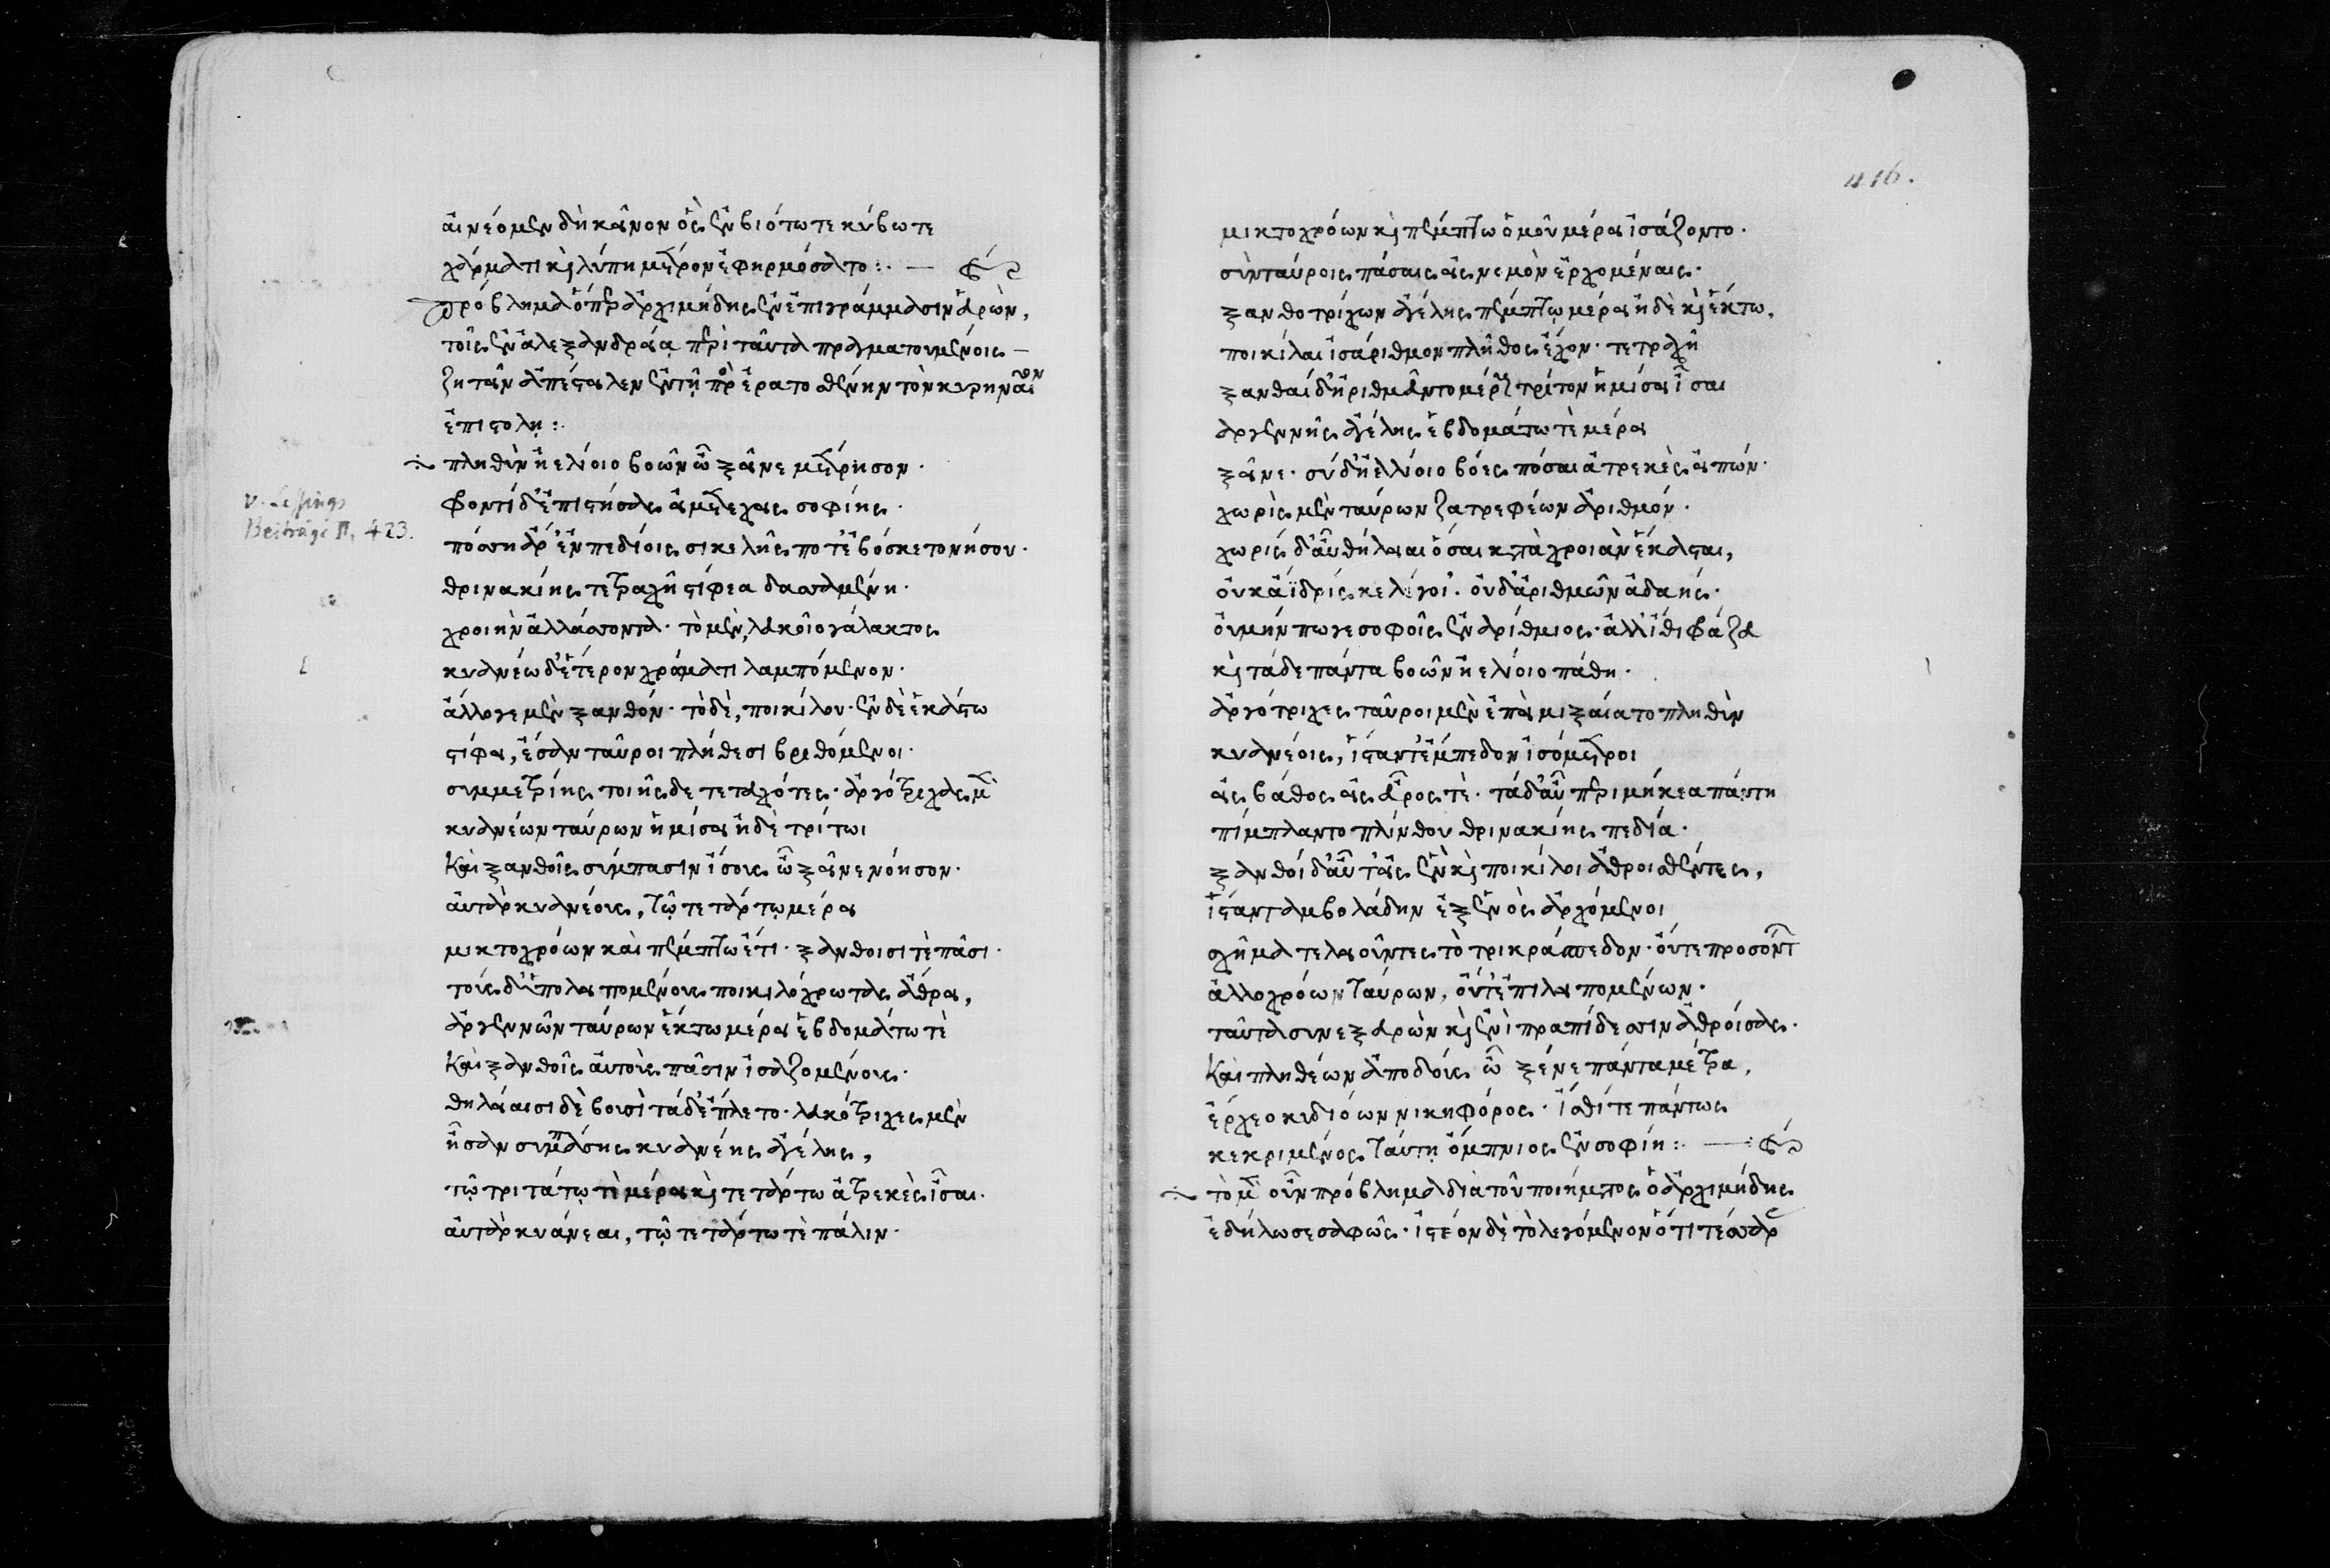
\includegraphics[scale=0.15]{images/cattle.jpeg}
   \caption{El manuscrito original con el problema del ganado de Arquímedes.}
   \label{fig:cattle}
\end{figure}

La primera solución al problema fue encontrada por Amthor en 1880. Amthor no
pudo calcular con exactitud estos números sino apenas conocer algunos de sus
dígitos. Estos números fueron encontrados en 1965 gracias al uso de
computadoras. 

%Hoy en día, para resolver la ecuación de Pell $x^2-Ny^2=1$, se considera
%el cuerpo $\Q(\sqrt{N})$, es decir el conjunto
%de números complejos de la forma
%\[
%	a+b\sqrt{N}
%\]
%donde $a$ y $b$ son números racionales. Cada elemento $\alpha=a+b\sqrt{N}$
%tiene una norma dada por $N(\alpha)=a^2-Nb^2$ y esta norma es una función
%multiplicativa, es decir
%\[
%	N(\alpha\beta)=N(\alpha)N(\beta)
%\]
%para todo $\alpha,\beta\in\Q(\sqrt{N})$. Encontrar entonces soluciones a la
%ecuación de Pell equivale a encontrar los elementos $\alpha=a+b\sqrt{N}$ con
%$a,b\in\Z$ y tal que $N(\alpha)=1$. 

%La identidad de Brahmugupta en el caso $N=-1$ nos da una fórmula para escribir
%el producto de dos sumas de cuadrados como una suma de cuadrados. De hecho,
%esta fórmula tiene puede expresarse simplemente así
%\[
%	|z_1z_2|^2=|z_1|^2|z_2|^2,\quad z_1,z_2\in\C.
%\]

\section*{Inducción matemática}

\index{Inducción!matemática}
\index{Inducción!demostrativa}
El método de Bhaskara nos sugiere cierta conexión con la inducción matemática
que comunmente utilizamos en algunas demostraciones.  Y ya que mencionamos la
inducción matemática, este parece ser un buen momento para hacer algunos
comentarios sobre las demostraciones por inducción. 

Nos basaremos en el
artículo~\cite{MR1519060}. 

Las demostraciones por inducción aparecen
independiente en trabajos de Pascal, Fermat y Maurolycus, aunque no siempre
presente de la forma en la que hoy la conocemos. Por ejemplo, en los trabajos
de Fermat aparece bajo una técnica que hoy conocemos como ``método del descenso''. 
%la técnica de Fermat consiste básicamente
%en asumir que si una cierta propiedad es válida para $n$, entonces será válida para $n-n_1$ y luego para $n-n_1-n_2$
Un proceso similar al descenso de Fermat había sido usado por Campanus en su
demostración de la irracionalidad del número $\frac{1+\sqrt{5}}{2}$ en su
edición de los elementos de Euclides del año 1260. Ninguno de los matemáticos
que utilzaron técnicas de demostración similares a la inducción consideraron
necesario asignarle un nombre especial. Wallis es uno de los primeros
matemáticos en utilizar oraciones como ``proceder por inducción'', aunque usaba
una inducción incompleta. Por ejemplo, en su libro de 1656, para demostrar que
\[
	\frac{1+4+9+\cdots+n^2}{(n+1)n^2}>\frac13
\]
calcula los primeros seis casos y afirma que esos casos son suficiententes para
entender qué pasa para otros valores de $n$. Jakob Bernoulli intenta en 1686
mejorar la técnica de Wallis y considera necesario agregar el argumento que
permite pasar del caso $n$ al caso $n+1$. Bernoulli no consideró necesario
asignarle un nombre especial a este procedimiento. En un libro póstumo
publicado en 1713 demuestra el teorema del binomio por inducción y lo hace con
las mejoras que introdujo anteriormente. Durante muchos de los años siguientes
los matemáticos utilizaron las técnicas de inducción de Wallis y de Bernoulli
indistintamente. A principios del siglo XVII varios diccionarios hablan de la
inducción en matemática y mencionan el teorema del binomio como un ejemplo de
aplicación.  En un diccionario matemático publicado en 1814 Barlow da una
definición formal del proceso de inducción:
\begin{quote}
	Induction is a term used by mathematicians to denote those of any law, or
	form, is inferred cases in which the generality from observing it to have
	obtained in several cases. Such inductions, however, are very deceptive,
	and ought to be admitted with the greatest caution.
\end{quote}
En 1830, el matemático inglés Peacock considera la inducción tal como fue
concebida por Bernoulli y la llama ``inducción demostrativa''. A partir de ese
momento la comunidad matemática poco a poco comienza a aceptar la noción de
inducción dada Bernoulli y olvida la inducción incompleta de Wallis.  En 1838,
De Morgan publicó un artículo sobre la inducción y la denominó ``inducción
matemática''. Muchos autores de libros de texto popularizaron estos nombres.
El famoso tratado sobre álgebra de Chrystal, por ejemplo, utiliza ``inducción
matemática''. Con el tiempo, esta terminología ganó terreno y poco a poco la
comunidad olvidó el nombre sugerido por Peacock. 


%\section*{El teorema de unidades de Dirichlet}
%
%En 1837 Dirichlet publicó una fórmula explícita para algunos ecuaciones de Pell. Por ejemplo, 
%para $N=13$, 
%\[
%	\eta^2=x_1+y_1\sqrt{13},
%\]
%donde 
%\[
%	\eta=\frac{\sin (2\pi/13) \sin(5\pi/13)\sin(6\pi/13)}{\sin(\pi/13)\sin (3\pi/13)\sin(4\pi/13)}\in\Q(\sqrt{13}).
%\]
%Resolver la ecuación de Pell en enteros positivos puede verse como un caso
%particular del teorema de las unidades de Dirichlet, demostrado en 1846. El teorema
%en el caso particular que mencionamos describe el grupo de unidades del anillo 
%de enteros algebraicos $\Z[\sqrt{N}]$. 
%
%En 1863 Kronecker publicó una expresión en términos de funciones elípticas. \framebox{?}
%
%
%
%
